\documentclass{article}

\setlength{\headsep}{0.75 in}
\setlength{\parindent}{0 in}
\setlength{\parskip}{0.1 in}

%=====================================================
% Add PACKAGES Here (You typically would not need to):
%=====================================================

\usepackage{xcolor}
\usepackage[margin=1in]{geometry}
\usepackage{amsmath,amsthm}
\usepackage{fancyhdr}
\usepackage{enumitem}
\usepackage{graphicx}
\usepackage{algorithmic}
\usepackage{algorithm}

\usepackage{amsmath, amssymb}  % Include the amsmath and amssymb packages for mathematical symbols

%=====================================================
% Ignore This Part (But Do NOT Delete It:)
%=====================================================

\theoremstyle{definition}
\newtheorem{problem}{Problem}
\newtheorem*{fun}{Fun with Algorithms}
\newtheorem*{challenge}{Challenge Yourself}
\def\fline{\rule{0.75\linewidth}{0.5pt}}
\newcommand{\finishline}{\begin{center}\fline\end{center}}
\newtheorem*{solution*}{Solution}
\newenvironment{solution}{\begin{solution*}}{{\finishline} \end{solution*}}
\newcommand{\grade}[1]{\hfill{\textbf{($\mathbf{#1}$ points)}}}
\newcommand{\thisdate}{February 29, 2024}
\newcommand{\thissemester}{\textbf{Rutgers: Spring 2024}}
\newcommand{\thiscourse}{ECE 509: Convex Optimization} 
\newcommand{\thishomework}{Number} 
\newcommand{\thisname}{Name} 
\newcommand{\thisextension}{Yes/No} 

\headheight 40pt              
\headsep 10pt
\renewcommand{\headrulewidth}{0pt}
\pagestyle{fancy}

\newcommand{\thisheading}{
   \noindent
   \begin{center}
   \framebox{
      \vbox{\vspace{2mm}
    \hbox to 6.28in { \textbf{\thiscourse \hfill \thissemester} }
       \vspace{4mm}
       \hbox to 6.28in { {\Large \hfill Homework \#\thishomework \hfill} }
       \vspace{2mm}
         \hbox to 6.28in { { \hfill \thisdate  \hfill} }
       \vspace{2mm}
       \hbox to 6.28in { \emph{Name: \thisname \hfill Extension: \thisextension}}
      \vspace{2mm}}
      }
   \end{center}
   \bigskip
}

%=====================================================
% Some useful MACROS (you can define your own in the same exact way also)
%=====================================================


\newcommand{\ceil}[1]{{\left\lceil{#1}\right\rceil}}
\newcommand{\floor}[1]{{\left\lfloor{#1}\right\rfloor}}
\newcommand{\prob}[1]{\Pr\paren{#1}}
\newcommand{\expect}[1]{\Exp\bracket{#1}}
\newcommand{\var}[1]{\textnormal{Var}\bracket{#1}}
\newcommand{\set}[1]{\ensuremath{\left\{ #1 \right\}}}
\newcommand{\poly}{\mbox{\rm poly}}


%=====================================================
% Fill Out This Part With Your Own Information:
%=====================================================


\renewcommand{\thishomework}{4} %Homework number
\renewcommand{\thisname}{Ravi Raghavan} % Enter your name here
\renewcommand{\thisextension}{No} % Pick only one of the two options accordingly

\begin{document}

\thisheading
\vspace{-0.75cm}


%=====================================================
% LaTeX Tip: You can erase this part from here.... 
%=====================================================		

\finishline

%=====================================================
% LaTeX Tip: ... to here
%=====================================================	


\bigskip

\begin{problem} \textit{Initial point and sublevel set condition.} Consider the function $f(x) = x_1^2 + x_2^2$ with domain $dom f = \{ (x_1, x_2) | x_1 > 1\}.$

\begin{enumerate}
    \item[(a)] What is $p^*$ and is it attained by any $x \in dom(f)$?
    \begin{solution}
        $p^* = \inf_x f(x) = \lim_{x\to (1, 0)} f(x) = 1$. Unfortunately, this is NOT attained by any $x \in dom(f)$
    \end{solution}
    \item[(b)] Draw the sublevel set $S = \{x | f(x) \leq f(x^{(0)})\}$ for $x^{(0)} = (2, 2)$. Is the sublevel set $S$ closed? Is $f$ strongly convex on $S$?
    \begin{solution}
        \begin{figure}[h!]
        \centering
        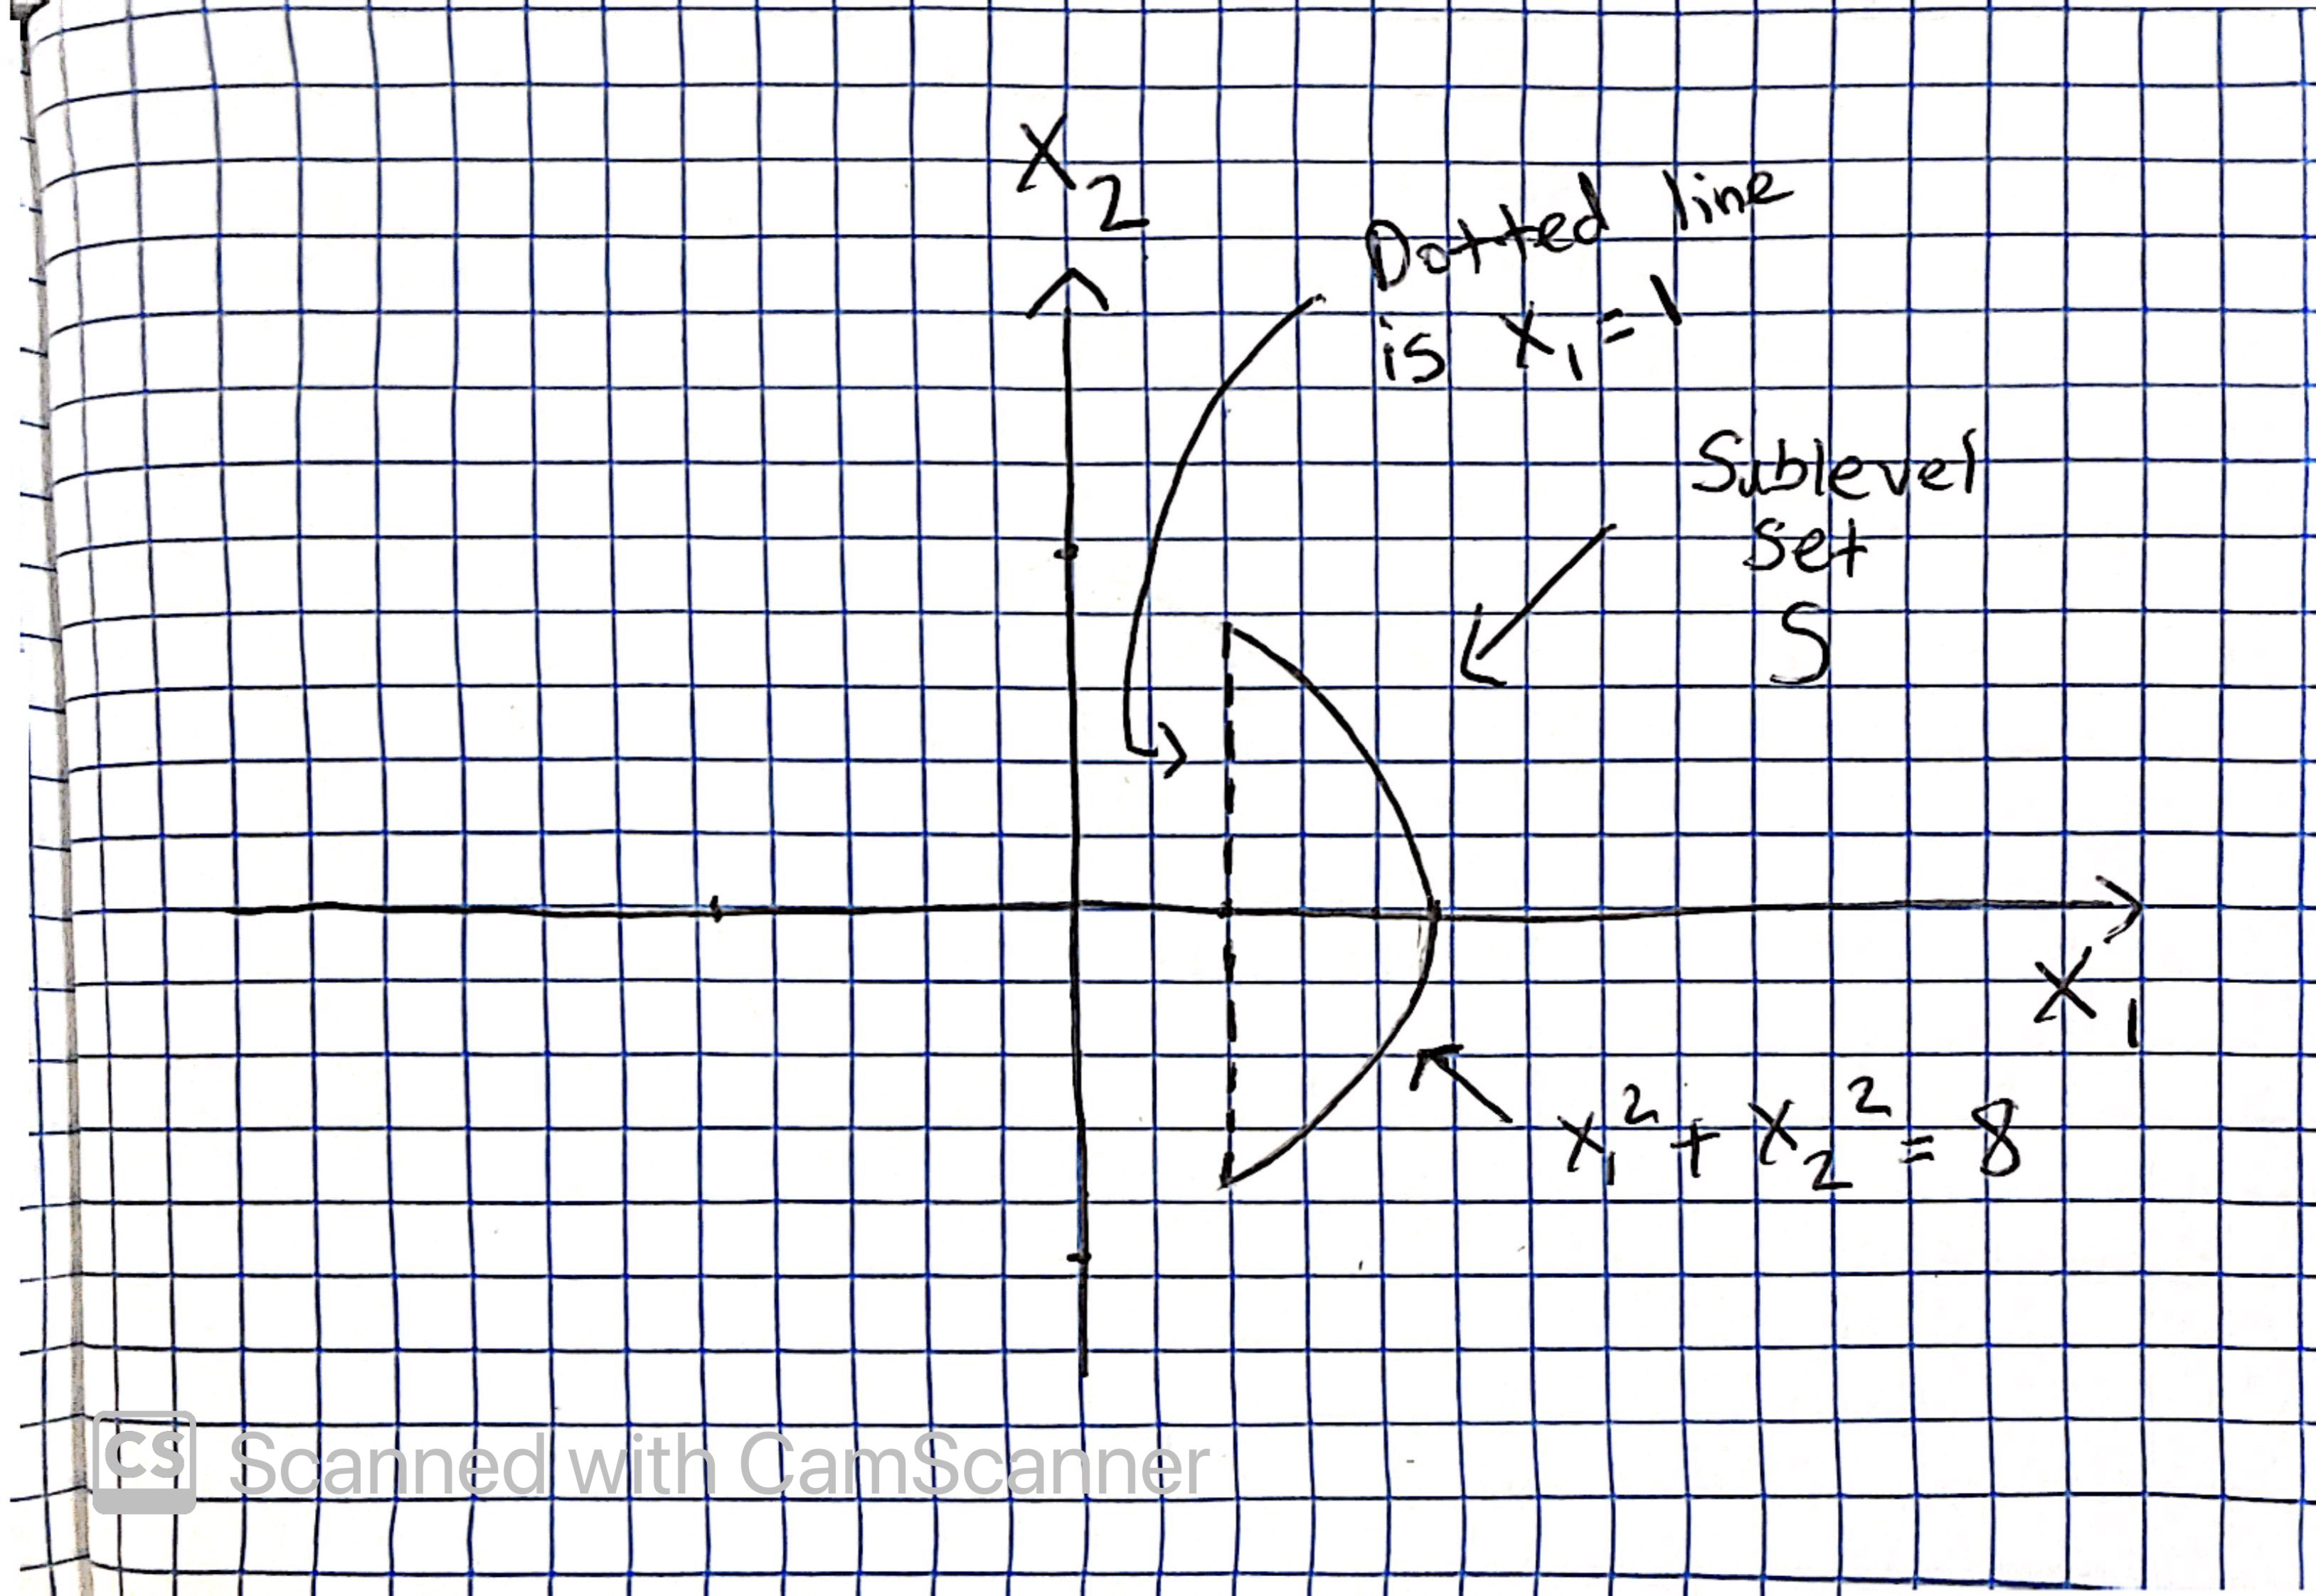
\includegraphics[width=\textwidth]{1b.jpg}
        \caption{Sketch of Sublevel Set}
    \end{figure}  
    \end{solution} Note: The sketch is on the next page

    This sublevel set is NOT closed. Let's look at the sequence $(\frac{t + 1}{t}, 1)$ for $t \in \mathbb{N}$. Please note that, in this definition, the Natural Numbers are $1, 2, 3, .....$. It DOES NOT include 0.  This sequence is contained within the sublevel set but, the limit point of $(1, 1)$ is NOT in the sublevel set
    
    $f$ IS strongly convex on $S$. $\nabla f(x) = \begin{pmatrix}
2x_1 \\
2x_2
\end{pmatrix}$, $\nabla^2 f(x) = \begin{pmatrix}
2 & 0 \\
0 & 2
\end{pmatrix}$. Hence, we can clearly find an $m$ and $M$ such that $mI \preceq \nabla^2 f(x) \preceq MI$

    \item[(c)] What happens if we apply the gradient method with backtracking line search, starting at $x^{(0)}$? Does $f(x^{(k)})$ converge to $p^*$? 

    \begin{solution}
    We can see that $\nabla f(x) = \begin{pmatrix}
2x_1 \\
2x_2
\end{pmatrix}$, $-\nabla f(x) = \begin{pmatrix}
-2x_1 \\
-2x_2
\end{pmatrix}$

Since $f$ is strongly convex on $S$, if we apply the backtracking line search starting at $x^{(0)}$, $f(x^{(k)})$ should converge to $p^*$
 
    \end{solution}
\end{enumerate}

    
\end{problem}

\newpage
\begin{problem} \textit{Backtracking Line Search} Suppose $f$ is strongly convex with $mI \preceq \nabla^2f(x) \preceq MI$. Let $\Delta x$ be a descent direction at $x$. Show that the backtracking stopping condition holds for

\begin{equation}
                        \label{eq:example}
                            0 < t \leq -\frac{\nabla f(x)^T \Delta x}{M ||\Delta x||^2_2}
                    \end{equation}

Use this to give an upper bound on the number of backtracking iterations. 

\begin{solution} Let's briefly revisit the backtracking algorithm 

\begin{algorithm}
\caption{Backtracking}
\begin{algorithmic} 
\STATE Parameters: $\Delta x$(Given Descent Direction for $f$ at $x \in dom f$) , $\alpha \in (0, 0.5)$, $\beta \in (0, 1)$
\STATE $t = 1$

\WHILE{$f(x + t\Delta x) > f(x) + \alpha t\nabla f(x)^T \Delta x$}
\STATE {$t = \beta t$ } 
\ENDWHILE

\end{algorithmic}
\end{algorithm}

Based on the definition of strong convexity, we know that \newline 
\begin{equation}
    \label{eq:example}
        f(y) \leq f(x) + \nabla f(x)^T (y - x) + \frac{M}{2} ||y - x||^2_2
\end{equation}

Hence, if we set $y = x + t\Delta x$ 
\begin{equation}
    \label{eq:example}
        f(x + t\Delta x) \leq f(x) + \nabla f(x)^T (x + t\Delta x - x) + \frac{M}{2} ||x + t\Delta x - x||^2_2
\end{equation}

\begin{equation}
    \label{eq:example}
        f(x + t\Delta x) \leq f(x) + t\nabla f(x)^T (\Delta x) + \frac{Mt^2}{2} ||\Delta x||^2_2
\end{equation}

Backtracking Stopping Condition: $f(x + t\Delta x) \leq f(x) + \alpha t\nabla f(x)^T (\Delta x)$ \newline 
Due to the definition of strong convexity, we are guaranteed for this backtracking stopping condition to hold when: \newline 
$f(x) + \alpha t\nabla f(x)^T (\Delta x) \geq f(x) + t\nabla f(x)^T (\Delta x) + \frac{Mt^2}{2} ||\Delta x||^2_2$ 

$\alpha t\nabla f(x)^T (\Delta x) \geq t\nabla f(x)^T (\Delta x) + \frac{Mt^2}{2} ||\Delta x||^2_2$

$0 \geq (1 - \alpha) t \nabla f(x)^T (\Delta x) + \frac{Mt^2}{2} ||\Delta x||^2_2$

$0 \geq t[(1 - \alpha) \nabla f(x)^T (\Delta x) + \frac{Mt}{2} ||\Delta x||^2_2]$

We must have $t > 0$ AND $(1 - \alpha) \nabla f(x)^T (\Delta x) + \frac{Mt}{2} ||\Delta x||^2_2 \leq 0$

$(1 - \alpha) \nabla f(x)^T (\Delta x) + \frac{Mt}{2} ||\Delta x||^2_2 \leq 0$ \newline 

$\frac{Mt}{2} ||\Delta x||^2_2 \leq (\alpha - 1) \nabla f(x)^T (\Delta x)$ \newline 

$t \leq \frac{2(\alpha - 1) \nabla f(x)^T (\Delta x)}{M||\Delta x||^2_2}$ \newline 



Since $\alpha \in (0, 0.5)$, we can see that $\frac{2(\alpha - 1) \nabla f(x)^T (\Delta x)}{M||\Delta x||^2_2} < -\frac{\nabla f(x)^T \Delta x}{M ||\Delta x||^2_2}$ \newline 

Hence, we see that $0 < t \leq -\frac{\nabla f(x)^T \Delta x}{M ||\Delta x||^2_2}$

Let $t_1 = -\frac{\nabla f(x)^T \Delta x}{M ||\Delta x||^2_2}$ \newline

For an upper bound on the number of backtracking iterations, we need: \newline 
$\beta^k \leq t_1$ \newline
$k \geq \log _{\beta}(t_1)$ \newline

\end{solution}
\end{problem}

\begin{problem} \textit{Quadratic problem in } $\mathbb{R}^2.$  Verify the expressions for the iterates $x^{(k)}$ in the first example of 9.3.2

\begin{solution} 
$f(x) = \frac{1}{2} (x_1^2 + \gamma x_2^2)$, $\frac{\partial{f}}{\partial{x_1}} = x_1$ and $\frac{\partial{f}}{\partial{x_2}} = \gamma x_2$, $\nabla f(x) = (x_1, \gamma x_2)$ \newline 

We know that, at $k = 0$, $x^0 = (\gamma, 1)$ \newline 


$x^{(k)} - \alpha \nabla f(x^{(k)}) = \begin{pmatrix}
(1 - \alpha) x_1 \\
(1 - \alpha \gamma) x_2
\end{pmatrix}$

\textbf{\underline{Exact Line Search:}} \newline 
Given the expressions for the iterates $x^{(k)}$, let's conduct exact line search. In the book, the iterate expressions are given as follows: \newline 

$x_1^{(k)} = \gamma (\frac{\gamma - 1}{\gamma + 1})^k$ and $x_1^{(k)} = (-\frac{\gamma - 1}{\gamma + 1})^k$

Substituting these expressions into $x^{(k)} - \alpha \nabla f(x^{(k)})$ gives us: \newline 

$x^{(k)} - \alpha \nabla f(x^{(k)}) = \begin{pmatrix}
(1 - \alpha) x_1 \\
(1 - \alpha \gamma) x_2
\end{pmatrix} = (\frac{\gamma - 1}{\gamma + 1})^k \begin{pmatrix}
(1 - \alpha) \gamma \\
(1 - \alpha \gamma) (-1)^k
\end{pmatrix}$ \newline 

$f(x^{(k)} - \alpha \nabla f(x^{(k)})) = \frac{1}{2} (\frac{\gamma - 1}{\gamma + 1})^{2k} ((1 - \alpha)^2 \gamma^2 + \gamma (1 - \alpha \gamma)^2)$ \newline 

To minimize $g(\alpha) = f(x^{(k)} - \alpha \nabla f(x^{(k)}))$, it is clear that we must minimize $((1 - \alpha)^2 \gamma^2 + \gamma (1 - \alpha \gamma)^2)$

$\frac{d}{d\alpha}((1 - \alpha)^2 \gamma^2 + \gamma (1 - \alpha \gamma)^2) = -2(1 - \alpha)\gamma^2 -2\gamma^2 (1 - \alpha \gamma)$ \newline 

Setting this derivative equal to 0 gives us: \newline 
$-2(1 - \alpha)\gamma^2 -2\gamma^2 (1 - \alpha \gamma) = 0$ \newline 
$-2\gamma^2 + 2\alpha \gamma^2 -2\gamma^2 + 2 \alpha \gamma^3 = 0$ \newline 

Divide this entire equation by $2\gamma^2$ \newline 
$-1 + \alpha - 1 + \alpha \gamma = 0$ \newline 
$\alpha + \alpha \gamma = 2$ \newline 
$\alpha = \frac{2}{1 + \gamma}$ \newline 

Substituting the value of alpha, we get: \newline
$x^{(k + 1)} = x^{(k)} - \alpha \nabla f(x^{(k)}) = \begin{pmatrix}
(1 - \alpha) x_1^{(k)} \\
(1 - \alpha \gamma) x_2^{(k)}
\end{pmatrix} = \begin{pmatrix}
\frac{\gamma - 1}{\gamma + 1} x_1^{(k)} \\
\frac{1 - \gamma}{\gamma + 1} x_2^{(k)}
\end{pmatrix}$ \newline 


\textbf{\underline{Verification:}} \newline 
First, we show that the closed form expressions are TRUE for $k = 0$ \newline
$x_1^{(0)} = \gamma = \gamma (\frac{\gamma - 1}{\gamma + 1})^0$, $x_2^{(0)} = 1 =(-\frac{\gamma - 1}{\gamma + 1})^0$, $f(x^{(0)}) = \frac{1}{2} (\gamma^2 + \gamma) = \frac{\gamma (\gamma + 1)}{2} = \frac{\gamma (\gamma + 1)}{2} (\frac{\gamma - 1}{\gamma + 1})^{(2 * 0)} = \frac{\gamma (\gamma + 1)}{2} (\frac{\gamma - 1}{\gamma + 1})^{0}$ \newline 


Now, assuming the closed form expressions are TRUE for $k$, show that they must be true for $k + 1$ \newline 
$x^{(k + 1)} = x^{(k)} - \alpha \nabla f(x^{(k)}) = \begin{pmatrix}
\frac{\gamma - 1}{\gamma + 1} x_1^{(k)} \\
\frac{1 - \gamma}{\gamma + 1} x_2^{(k)}
\end{pmatrix} = \frac{\gamma - 1}{\gamma + 1} \begin{pmatrix}
    x_1^{(k)} \\
    -x_2^{(k)}
\end{pmatrix}$

$x_1^{(k + 1)} = \frac{\gamma - 1}{\gamma + 1} x_1^{(k)} = \frac{\gamma - 1}{\gamma + 1} (\gamma (\frac{\gamma - 1}{\gamma + 1})^k) = \gamma (\frac{\gamma - 1}{\gamma + 1})^{(k + 1)}$

$x_2^{(k + 1)} = \frac{\gamma - 1}{\gamma + 1} (-x_2^{(k)}) = -\frac{\gamma - 1}{\gamma + 1} (-\frac{\gamma - 1}{\gamma + 1})^k = (-\frac{\gamma - 1}{\gamma + 1})^{(k + 1)}$

$f(x^{(k + 1)}) = \frac{1}{2} (\frac{\gamma - 1}{\gamma + 1})^{2(k + 1)} (\gamma^2 + \gamma) = \frac{\gamma (\gamma + 1)}{2} (\frac{\gamma - 1}{\gamma + 1})^{2(k + 1)}$ \newline 



This completes the verification and shows that the following are TRUE: \newline 
$x_1^{(k)} = \gamma (\frac{\gamma - 1}{\gamma + 1})^{(k)}$ \newline 
$x_2^{(k)} = (-\frac{\gamma - 1}{\gamma + 1})^{(k)}$ \newline 
$f(x^{(k)}) = \frac{\gamma (\gamma + 1)}{2} (\frac{\gamma - 1}{\gamma + 1})^{2k}$

\end{solution}
\end{problem}

\end{document}





